\documentclass{article}

\usepackage{graphicx}
\graphicspath{{./graphics/}}
\usepackage{amsmath}

\usepackage[margin=2.5cm]{geometry}
\usepackage[margin=1cm]{caption}
\usepackage{pdfpages}

\title{EG2 DATA MINING ANALYSIS NOTE: \\
Ratio of $A(e,e'pp)$ to $A(e,e'p)$ events in SRC kinematics}

\author{A. Schmidt, et al.}

\begin{document}

\maketitle

\section{Introduction}

We present an analysis of the ratio of $A(e,e'pp)$ to $A(e,e'p)$ events in kinematics
dominated by the break-up of short-range correlated (SRC) pairs. We follow the same
procedure as in the previously approved CLAS analysis of reference~\cite{Or:note},
with a few refinements: the addition of approved fiducial cuts \cite{Lamiah:note} 
for protons, as well as implementing select kinematic corrections (following~\cite{Barak:note}).
Event selection of $A(e,e'pp)$ and $A(e,e'p)$ events is the same as in~\cite{Or:note}.
We compare the ratio of $A(e,e'pp)$ to $A(e,e'p)$ events to that predicted by a new 
Monte Carlo event generator using a theoretical framework 
called ``Generalized Contact Formalism'' (see \cite{weiss:2016obx,Weiss:2018tbu} for
details on the formalism). 

\subsection{Kinematic definitions used in this note}

\begin{figure}[htpb]
\centering
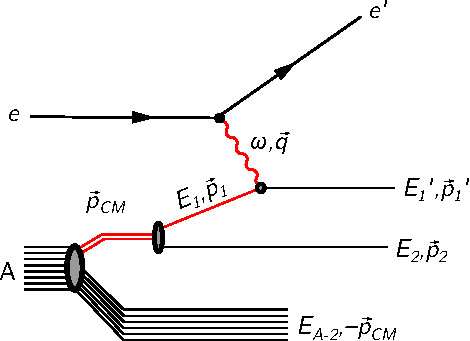
\includegraphics{reaction.pdf}
\caption{
Our event generator assumes this reaction, where the internal off-shell lines are
denoted in red.
\label{fig:reaction}}
\end{figure}

As shown in figure \ref{fig:reaction}, the relevant reaction involves electron
scattering and transferring energy $\omega$ and momentum, $\vec{q}$ to a proton
in an SRC pair, which had energy $E_1$ and momentum $\vec{p}_1$ prior to the
scattering, and has energy $E_1' = E_1 + \omega$ and momentum $\vec{p}_1' = \vec{p}_1 + \vec{q}$
after the scattering. The correlated partner nucleon recoils from the nucleus with
energy $E_2$ and momentum $\vec{p}_2$. No energy or momentum are transferred to the
partner nucleon during the scattering. Collectively, the nucleons in the pair have
center-of-mass momentum $\vec{p}_{CM} = \vec{p}_1 + \vec{p}_2$, and this is balanced
by the momentum of the residual $A-2$ system. The nucleons in the pair also have
relative momentum, $\vec{p}_\text{rel} \equiv (\vec{p}_1 - \vec{p}_2)/2$.

In the absence of final-state interactions, the initial momentum of the struck proton, $\vec{p}_1$,
is equal to the missing momentum, $\vec{p}_\text{miss} \equiv \vec{p}_1' - \vec{q}$. 
For that reason, we use $\vec{p}_\text{miss}$ as a proxy for $\vec{p}_1$.

We define missing energy, $E_\text{miss}$, as
\begin{equation}
E_\text{miss} = \omega - T_p - T_{A-1},
\end{equation}
where $T_p$ is the kinetic energy of the leading proton and $T_{A-1}$ is given by:
\begin{equation}
T_{A-1} = \omega + m_A - E_p - \sqrt{(\omega + m_A - E_p)^2 - p_\text{miss}^2}.
\end{equation}
We also make use of $M_\text{miss}$, which we define as:
\begin{equation}
  M_\text{miss}^2 = (q^\mu + 2 m_N - p_1'^{\mu})^2,
\end{equation}
where $m_N$ is the nucleon mass. This formulation of $M_\text{miss}$ assumes striking
a stationary SRC pair, i.e. $\vec{p}_{CM}=0$, and estimates the mass of the spectator
nucleon. 

\section{Kinematic Corrections}

While the event selection of this analysis is nearly identical to that of reference
\cite{Or:note}, we make use of kinematic corrections to improve the accuracy of the
reconstruction. First, we updated the EG2 beam energy to reflect the more accurate value
determined from Hall A measurements, presented in approved the approved EG2 analysis
described in reference \cite{Barak:note}. Rather than assuming the set value of 
of 5.014~GeV, we used the measured value of 5.009.4~GeV when calculating all derived
kinematic quantities. 

Next, we corrected the reconstructed polar angles ($\theta$) of all
particles, according to the correction for quasielastic kinematics derived in 
\cite{Barak:note}. These corrections were derived by looking at angle-angle 
correlations in hydrogen elastic data, and were found to vary as a function
of $\phi$ but not theta, see figure~\ref{fig:theta_corr}. We applied these 
exact corrections to both electrons and protons in our data. 

\begin{figure}[p]
\centering
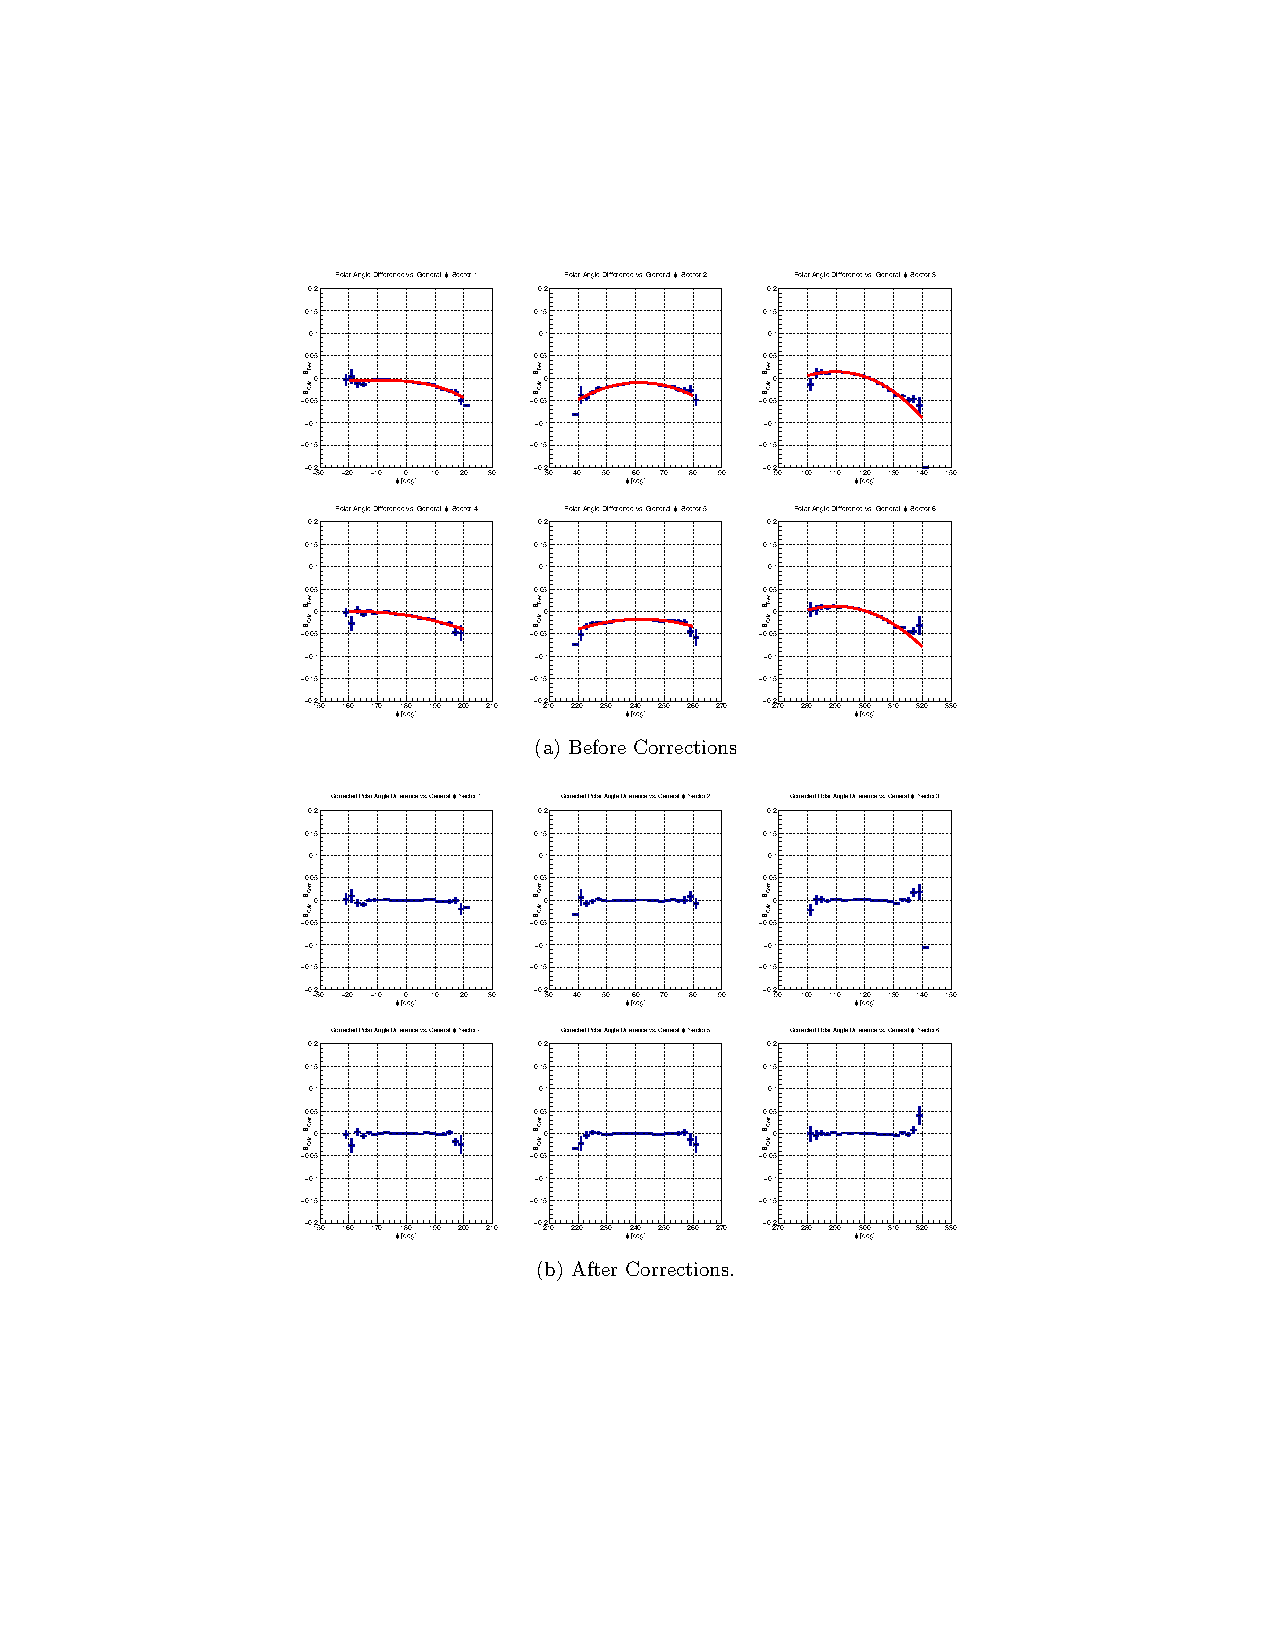
\includegraphics{barak_theta_corr.pdf} 
\caption{
These plots, taken directly from \cite{Barak:note}, show before and after $\theta$ 
corrections in hydrogen elastic data as a function of $\phi$. 
\label{fig:theta_corr}}
\end{figure}

Following $\theta$ corrections, we applied a correction to the reconstructed electron momentum, as a function
of sector. Such a correction was discussed in \cite{Barak:note}, but since the correction
was less than 20~MeV, it was deemed unneccesary for that analysis. We find that missing
energy distribution is sensitive to such effects, and opted to determine and apply
momentum corrections.

To determine such corrections, we looked deuterium $d(e,e'p)$ data. In quasielastic
break-up of the deuteron, there is an undetected neutron and so energy and momentum 
conservation require:
\begin{align}
p_n^mu &= q^\mu + p_d^\mu - p_p^\mu,\\
m_n^2 &= -Q^2 + 2\omega m_d - 2 q_\mu p_p^\mu + m_d^2 - 2 m_d E_p + m_p^2.
\end{align}
This can be rearranged to solve for the scattered electron momentum:
\begin{equation}
p_e = \frac{m_d^2 + m_p^2 - m_n^2 + 2(E_\text{beam}m_d - E_\text{beam} E_p + \vec{p}_\text{beam}\cdot\vec{p}_p - E_pm_d)}
{2(E_\text{beam} ( 1 - \cos\theta_e) + m_d - E_p + p_p \cos\theta_{ep})}
\end{equation}
Using this equation we can predict the electron momentum as a function of 
the electron angles, proton angles, and proton momentum.

To select quasielastic break-up events, we required that there be one electron
and one proton, and that:
\begin{itemize}
\item $|z_e - z_p| < 1.5$~cm, to reduce random background
\item $x_B > 0.85$, to reduce inelastic contribution.
\end{itemize}
We then compared the measured electron momentum to the expected momentum by electron
sector and fit the peak to determine the correction. The results are shown in figure
\ref{fig:E_corr}. We saw little evidence of $\theta$ or momentum dependence on the
size of this correction, and so applied the correction as a constant shift. The
effect on the missing energy distribution is shown in figure \ref{fig:Emiss_2d}.
The corrections used are given in table \ref{tab:Ecorr}.

\begin{table}[htb]
\centering
\begin{tabular}{c c c}
\hline
\hline
Sector & Central $\phi$ & Correction [MeV$/c$]\\
\hline
0 & $0^\circ$ &  6.64 \\
1 & $60^\circ$ & -21.07 \\
2 & $120^\circ$ & 5.19\\
3 & $180^\circ$ & 25.96\\
4 & $240^\circ$ & 3.62\\
5 & $300^\circ$ & -9.42\\
\hline
\end{tabular}
\caption{Corrections applied to reconstructed electron momenta, by sector \label{tab:Ecorr}}
\end{table}


\begin{figure}[p]
\centering
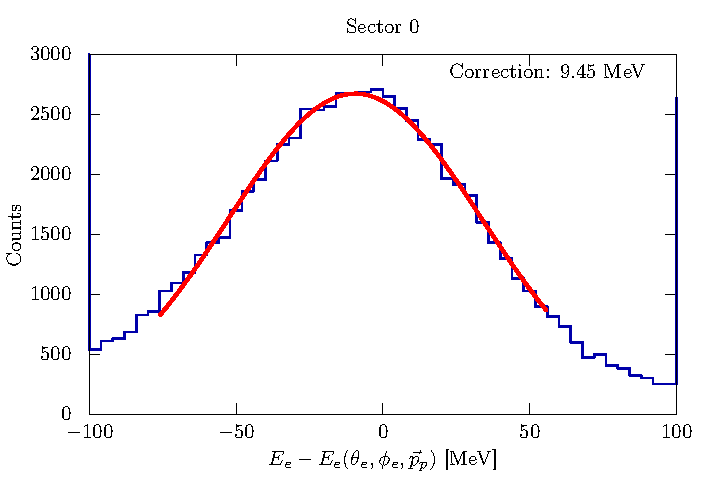
\includegraphics[width=0.49\textwidth]{Ecorr/corr_0.pdf}
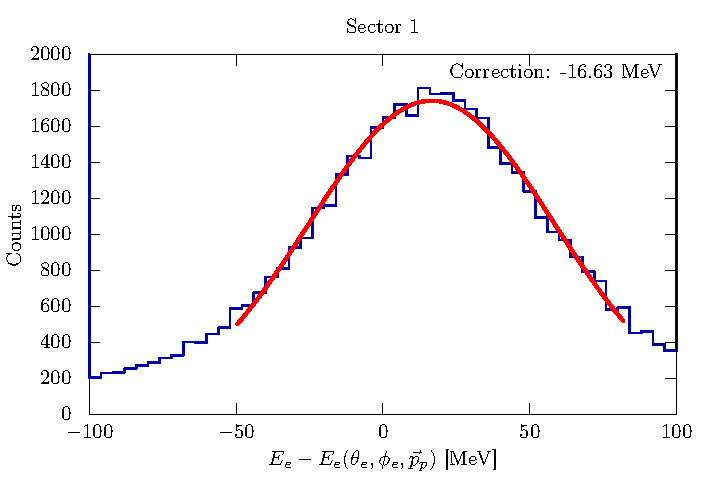
\includegraphics[width=0.49\textwidth]{Ecorr/corr_1.pdf}\\
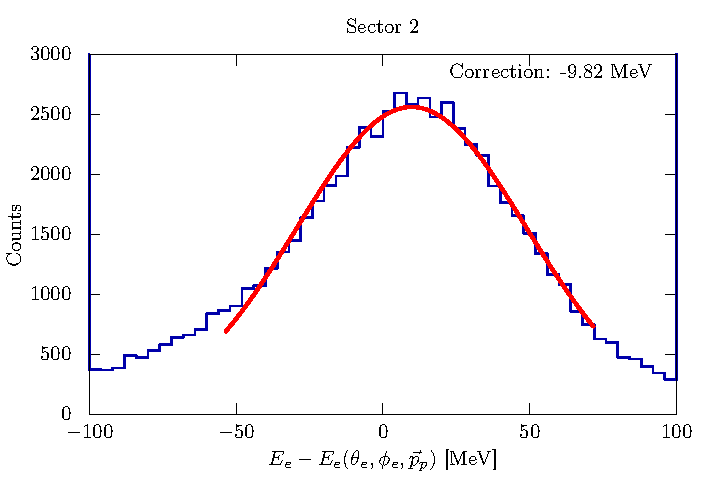
\includegraphics[width=0.49\textwidth]{Ecorr/corr_2.pdf}
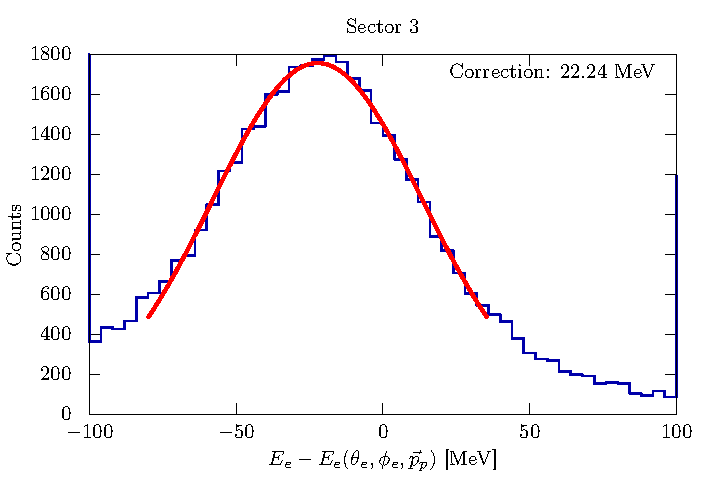
\includegraphics[width=0.49\textwidth]{Ecorr/corr_3.pdf}\\
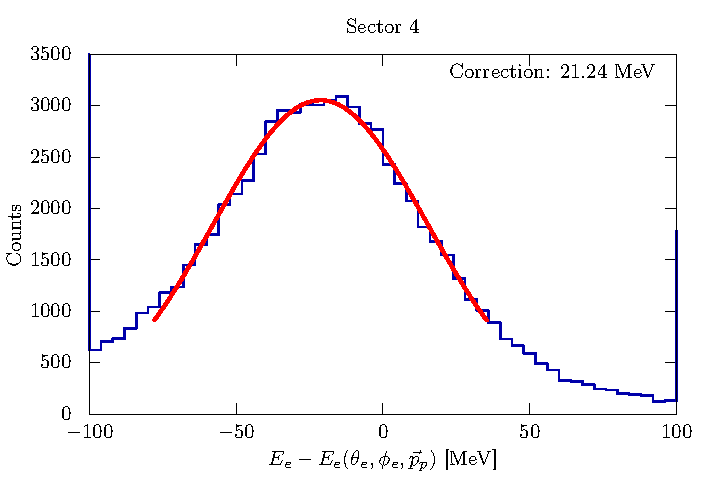
\includegraphics[width=0.49\textwidth]{Ecorr/corr_4.pdf}
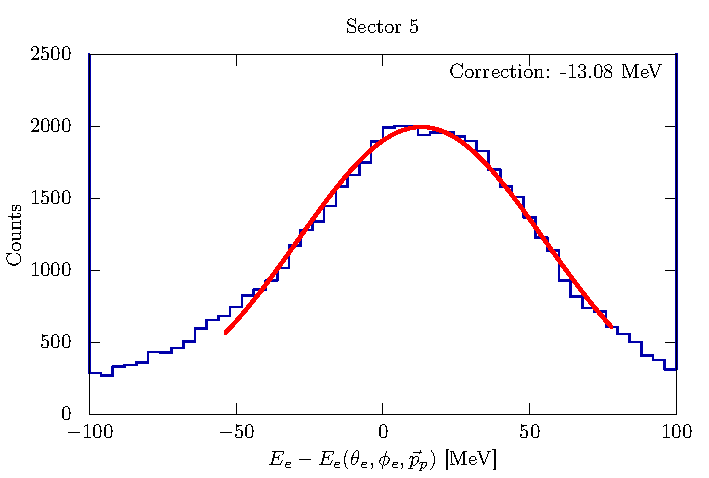
\includegraphics[width=0.49\textwidth]{Ecorr/corr_5.pdf}\\
\caption{
The electron momentum corrections were determined from $d(e,e'p)$ data for each sector.
\label{fig:E_corr}}
\end{figure}

\begin{figure}[p]
\centering
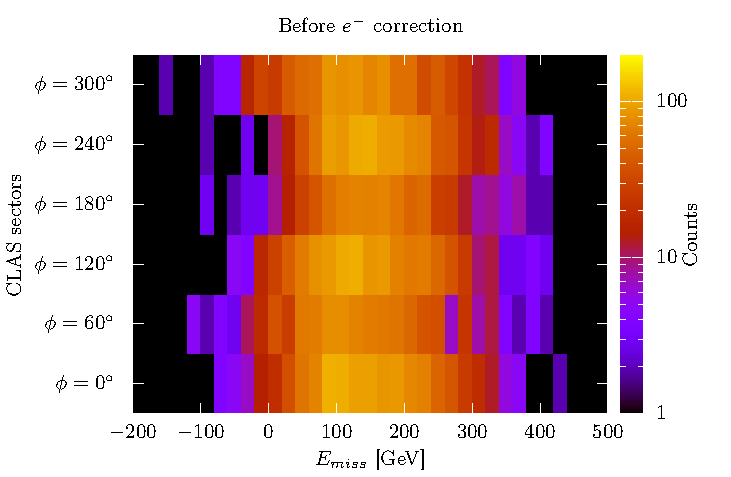
\includegraphics{Ecorr/Emiss_2d_uncorr.pdf}\\
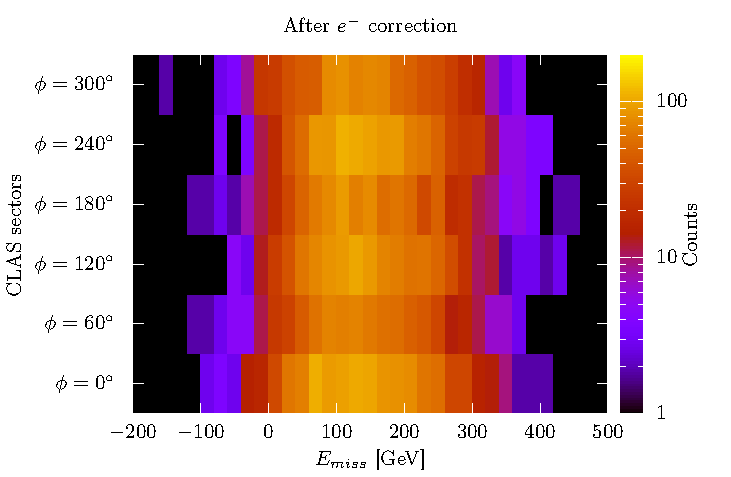
\includegraphics{Ecorr/Emiss_2d_corr.pdf}
\caption{
The electron corrections reduced the differences in the missing energy distribution
by sector (shown here for $C(e,e'p)$ data).
\label{fig:Emiss_2d}}
\end{figure}

\section{Event Selection}
\label{sec:data}

The event selection used in this analysis is nearly identical to that of the 
previously approved analysis ``Probing $pp$-SRC in $^{12}$C, $^{27}$Al, $^{56}$Fe, and $^{208}$Pb 
using the $A(e,e'p)$ and $A(e,e'pp)$ Reactions'' \cite{Or:note}. We recapitulate
the event selection cuts of that analysis here, and then discuss the additional
requirements that have been added for this analysis. 

In the analysis of \cite{Or:note}, the event selection criteria for ``Leading proton events,'' 
i.e., $A(e,e'p)$ events, were:
\begin{itemize}
\item $x_B > 1.2$
\item 0.3~GeV$/c$~$< |\vec{p}_\text{miss}| < 1$~GeV$/c$
\item $\theta_{pq} < 25^\circ$ and $0.62 < |\vec{p}_p|/|\vec{q}| < 0.96$ (shown in figure \ref{fig:p_over_q})
\item $M_\text{miss} < 1.1$ (shown in figure \ref{fig:m_miss})
\item $|\vec{p}_p| < 2.4$~GeV$/c$
\item $-25 < z_e < -20$~cm
\item $-25 < z_p < -20$~cm
\item $e^-$ fiducial cuts (shown in figure \ref{fig:e_fid})
\end{itemize}
No events had more than one proton passing leading proton cuts.


\begin{figure}[htpb]
\centering
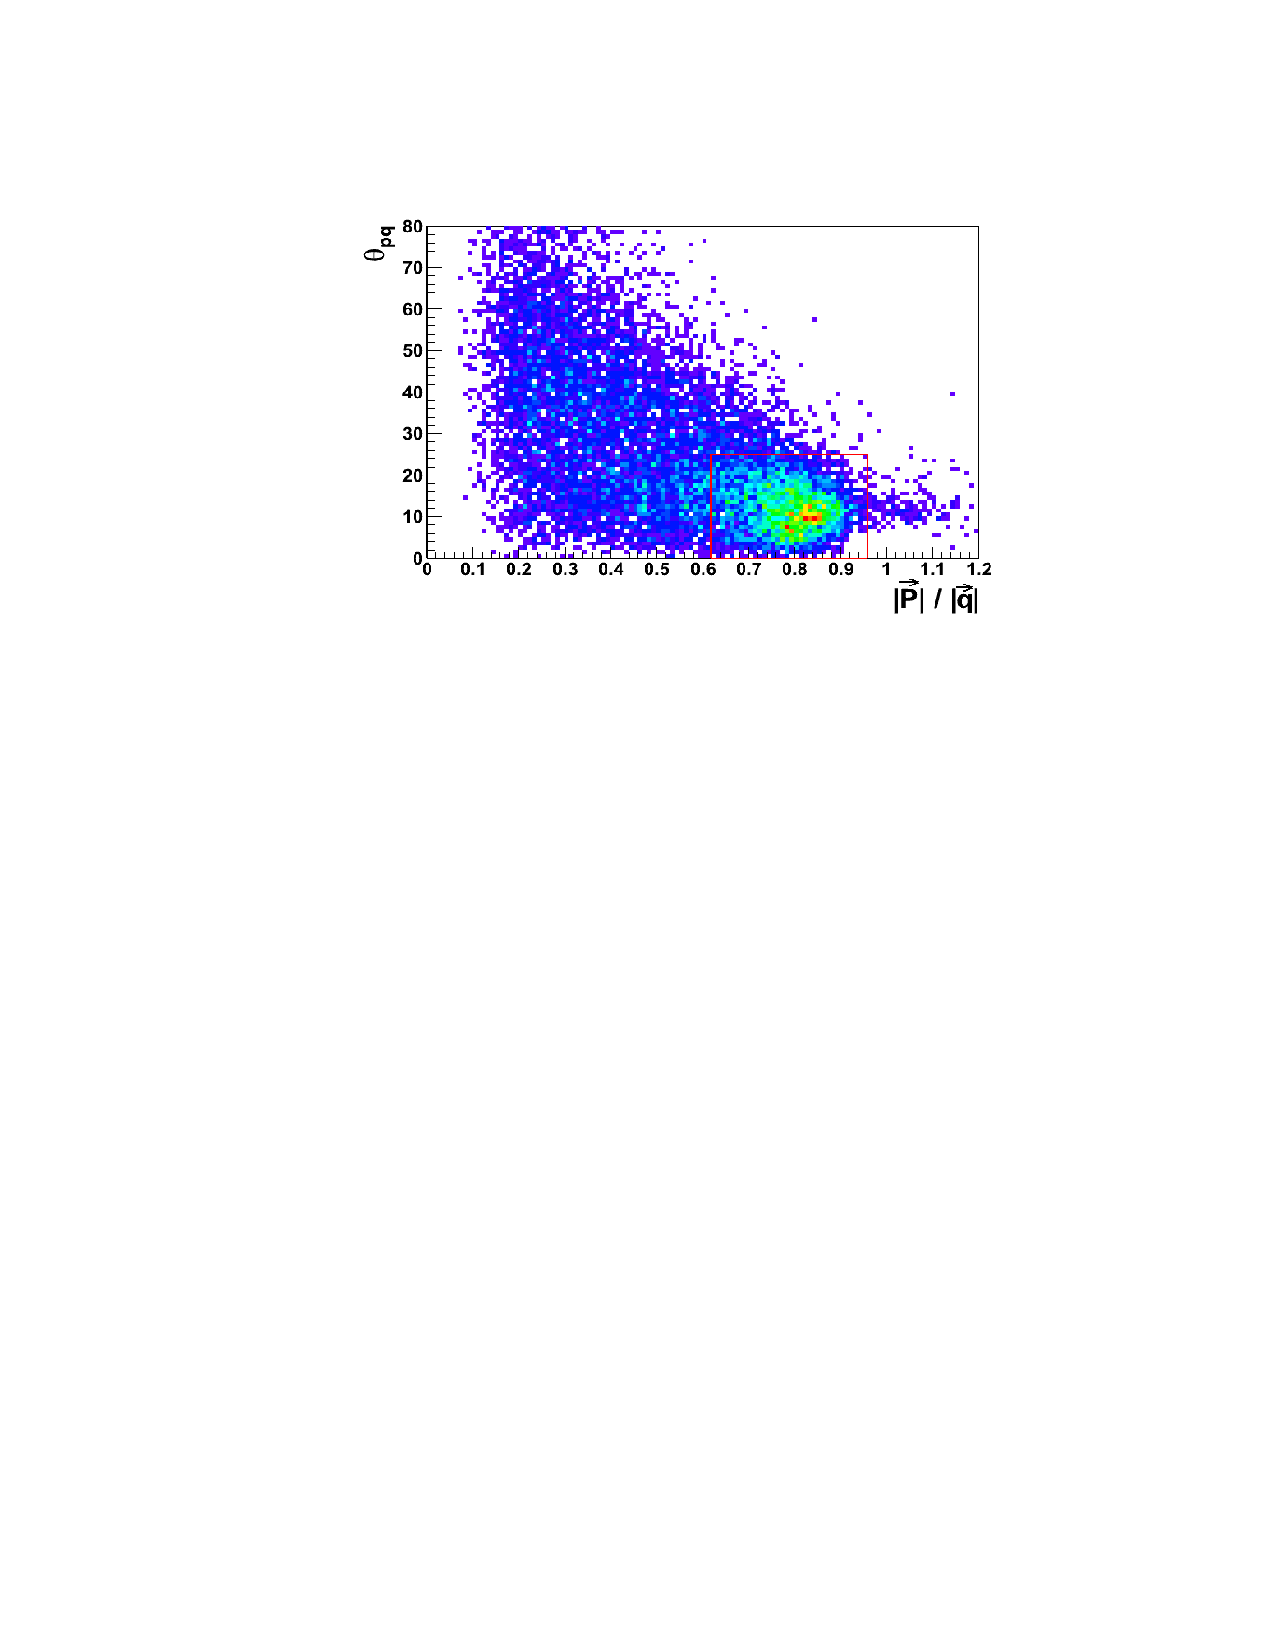
\includegraphics{or_note_figs/leading_selection.pdf}
\caption[$|\vec{p}_p|/|\vec{q}|$ and $\theta_{pq}$ cuts for leading protons]{
To pass leading cuts, the proton needed to emerge in the direction of the
momentum transfer, with $0.62 < |\vec{p}_p|/|\vec{q}| < 0.96$, as shown by the red
box. This figure was taken directly from reference~\cite{Or:note}.
\label{fig:p_over_q}}
\end{figure}

\begin{figure}[htpb]
\centering
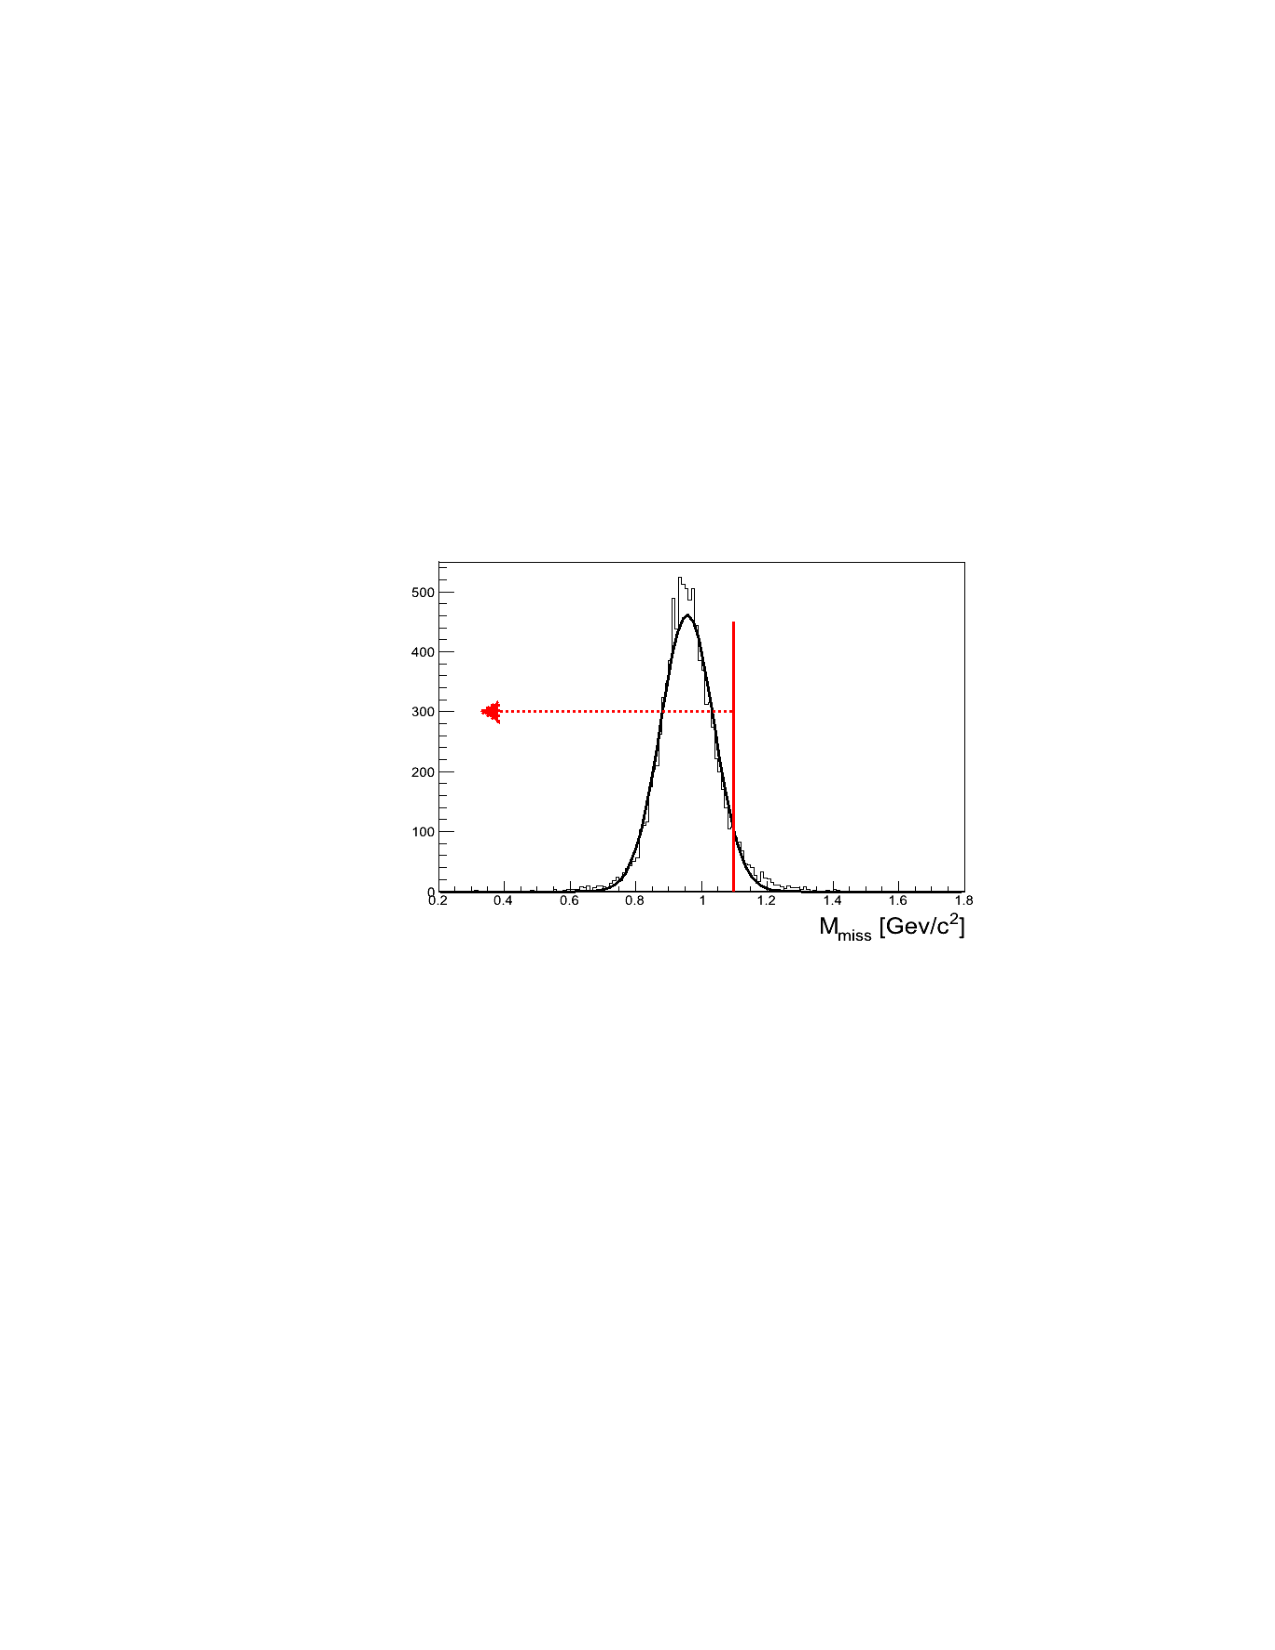
\includegraphics{or_note_figs/m_miss.pdf}
\caption[Missing mass cut]{
To pass leading cuts, the proton needed to emerge with missing mass less than
960~MeV$+m_\pi=1100$~MeV. This figure was taken directly from reference~\cite{Or:note}.
\label{fig:m_miss}
}
\end{figure}

\begin{figure}[htpb]
\centering
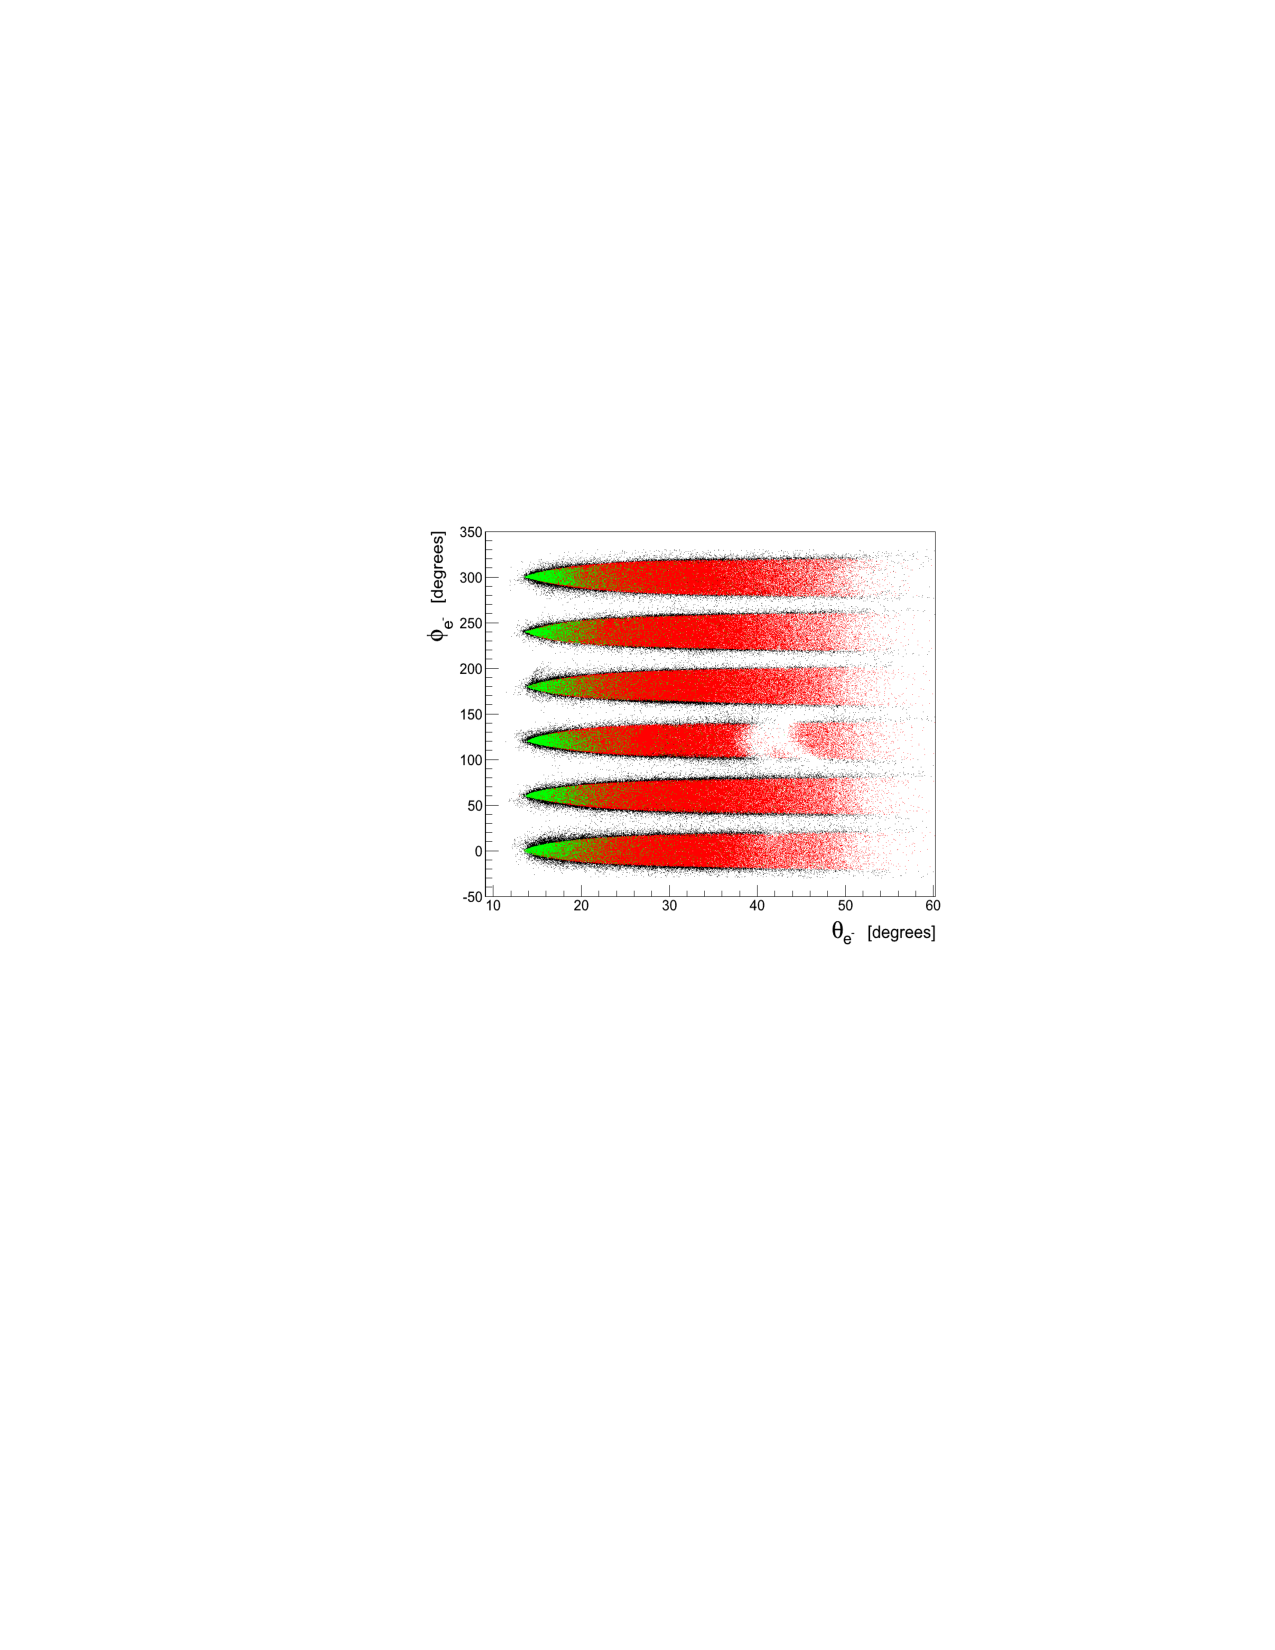
\includegraphics{or_note_figs/e_fid.pdf}
\caption[Electron fiducial cuts]{
The $\theta$ and $\phi$ angles for all electrons are shown in black. Those with
$x_B>1.2$ are shown in red, and those passing fiducial cuts are shown in green.
This figure was taken directly from reference~\cite{Or:note}.
\label{fig:e_fid}}
\end{figure}

Out of these $A(e,e'p)$ events, $A(e,e'pp)$ events were selected by matching the additional criteria:
\begin{itemize}
\item $|\vec{p}_\text{rec.}| > 0.35$~GeV$/c$
\item $-25 < z_\text{rec.} < -20$~cm
\end{itemize}

\subsection{Additional selection criteria}
We make two small modifications to the event selection of \cite{Or:note}:
\begin{itemize}
\item We restrict the missing momentum range to 0.4~GeV$/c$~$< |\vec{p}_\text{miss}| < 1$~GeV$/c$:
  we are comparing to an asymptotic theory valid at high missing momentum.
\item We require that all protons pass approved fiducial cuts.
\end{itemize}

\subsection{Proton fiducial cuts}

We use approved positive particle fiducial cuts developed in reference
\cite{Lamiah:note} (and subsequently used in approved SRC analysis of reference \cite{Erez:note}). 
The effect of the fiducial cuts can be seen in figures \ref{fig:lead_fid} and \ref{fig:recoil_fid}.

\begin{figure}[h]
\centering
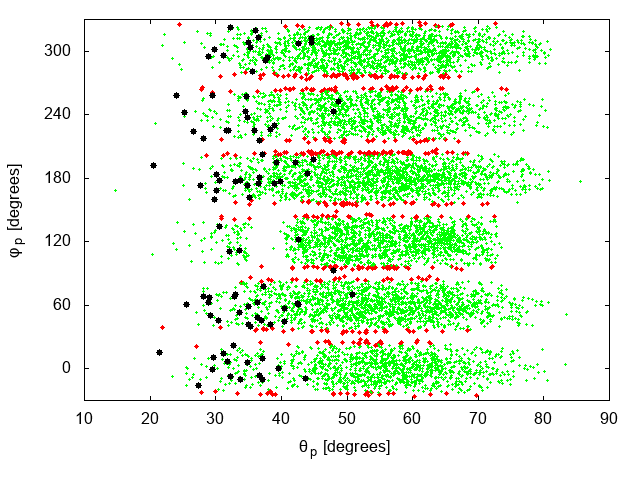
\includegraphics[width=0.55\textwidth]{lead_fid.png}
\caption[Leading proton fiducial cuts]{
The $\theta$ and $\phi$ angles for protons passing all leading cuts except for $|\vec{p}|<2.4$~GeV$/c$ are shown in black. Those 
failing failing proton fiducial cuts are shown in red. Protons passing leading cuts are shown in green. Events here are 
from the carbon target. 
\label{fig:lead_fid}}
\end{figure}

\begin{figure}[h]
\centering
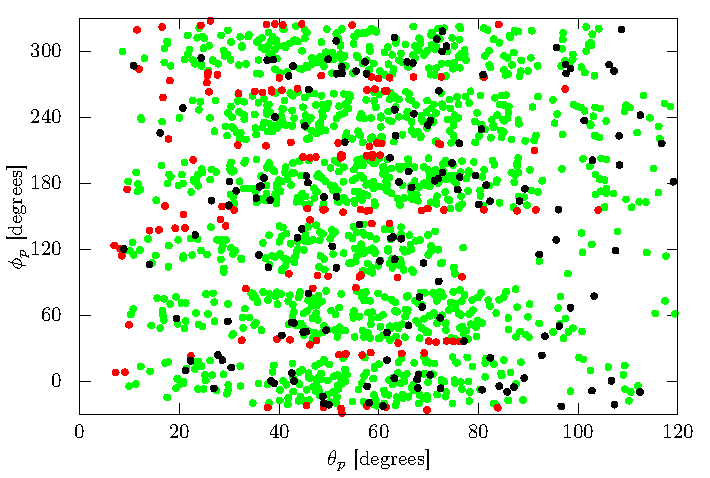
\includegraphics[width=0.55\textwidth]{recoil_fid.pdf}
\caption[Fiducial cuts for recoil protons]{
The $\theta$ and $\phi$ angles for recoil protons passing all cuts except for $|\vec{p}|>350$~MeV$/c$ are shown in black. Those 
failing failing proton fiducial cuts are shown in red. Protons passing all recoil cuts are shown in green. Events here are 
from the all four targets combined together. 
\label{fig:recoil_fid}
}
\end{figure}

\section{Distributions of selected Events}

\subsection{$A(e,e'p)$ events}

Table \ref{tab:leading} shows the number of events passing leading proton cuts, binned by missing
momentum.

\begin{table}[h]
\centering
\begin{tabular}{c c c c c}
\hline
\hline
$p_\text{miss}$ [GeV$/c$] & C Events & Al Events & Fe Events & Pb Events\\
\hline

0.3--0.4 & 3321  & 1048 & 3408 & 947  \\
0.4--0.5 & 2406  & 848  & 2802 & 874 \\
0.5--0.6 & 1919  & 690  & 2379 & 769  \\
0.6--0.7 & 963   & 361  & 1332 & 457  \\
0.7--0.8 & 383   & 162  &  501 & 153  \\
0.8--0.9 & 142   & 51   &  218 &  57 \\
0.9--1.0 & 41    & 24   &  78  &  30 \\
\hline
Total & 9175 & 3184 & 10718 & 3287 \\
\hline
\end{tabular}
\caption{\label{tab:leading} Events passing leading proton cuts; the numbers of events are smaller
than in table VII of \cite{Or:note} because of the additional proton fiducial cuts.}
\end{table}


\begin{figure}[htpb]
\centering
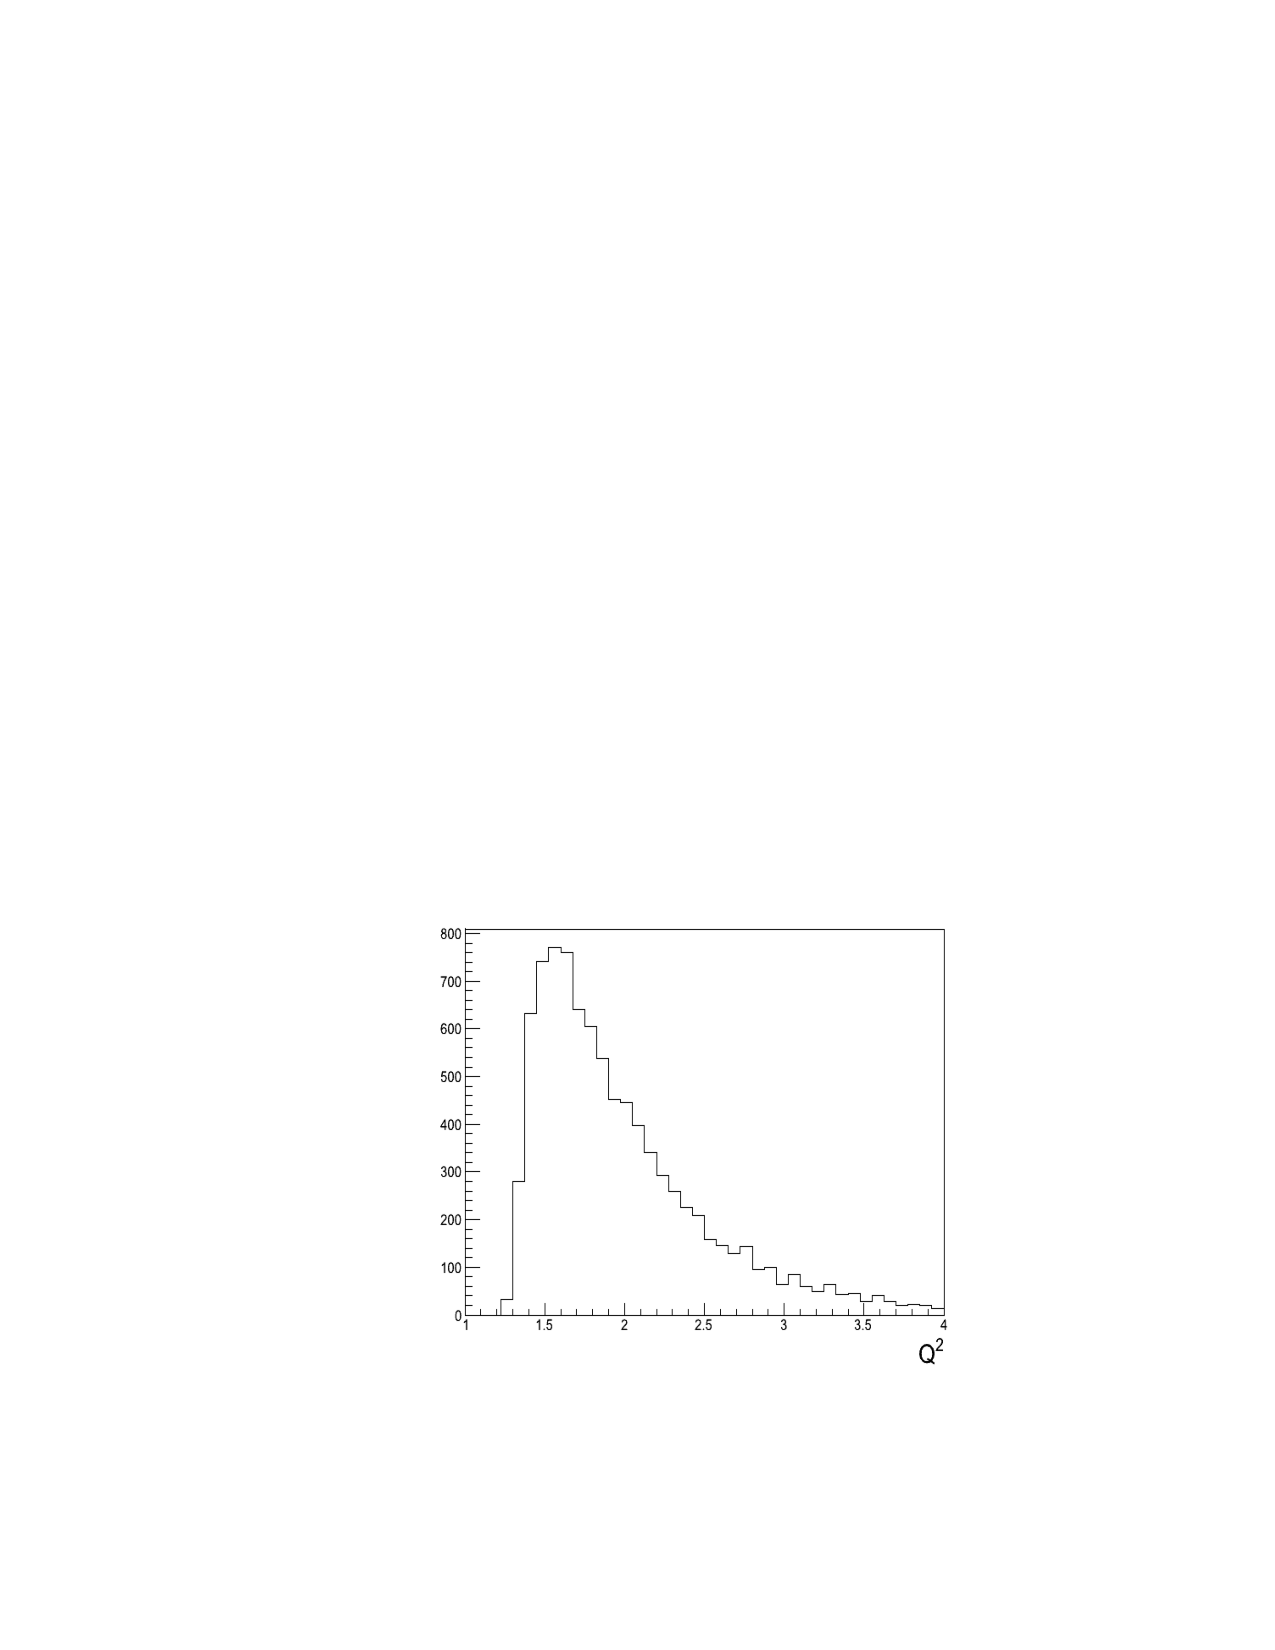
\includegraphics[width=0.43\textwidth]{or_note_figs/q2.pdf}
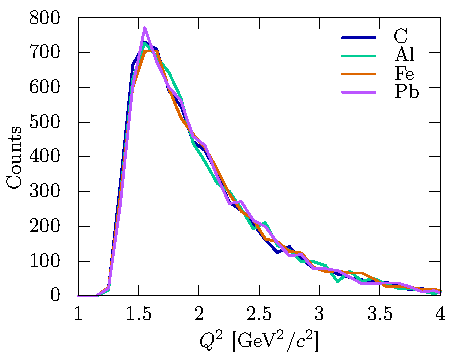
\includegraphics[width=0.49\textwidth]{leading_dist/leading_QSq.pdf}\\
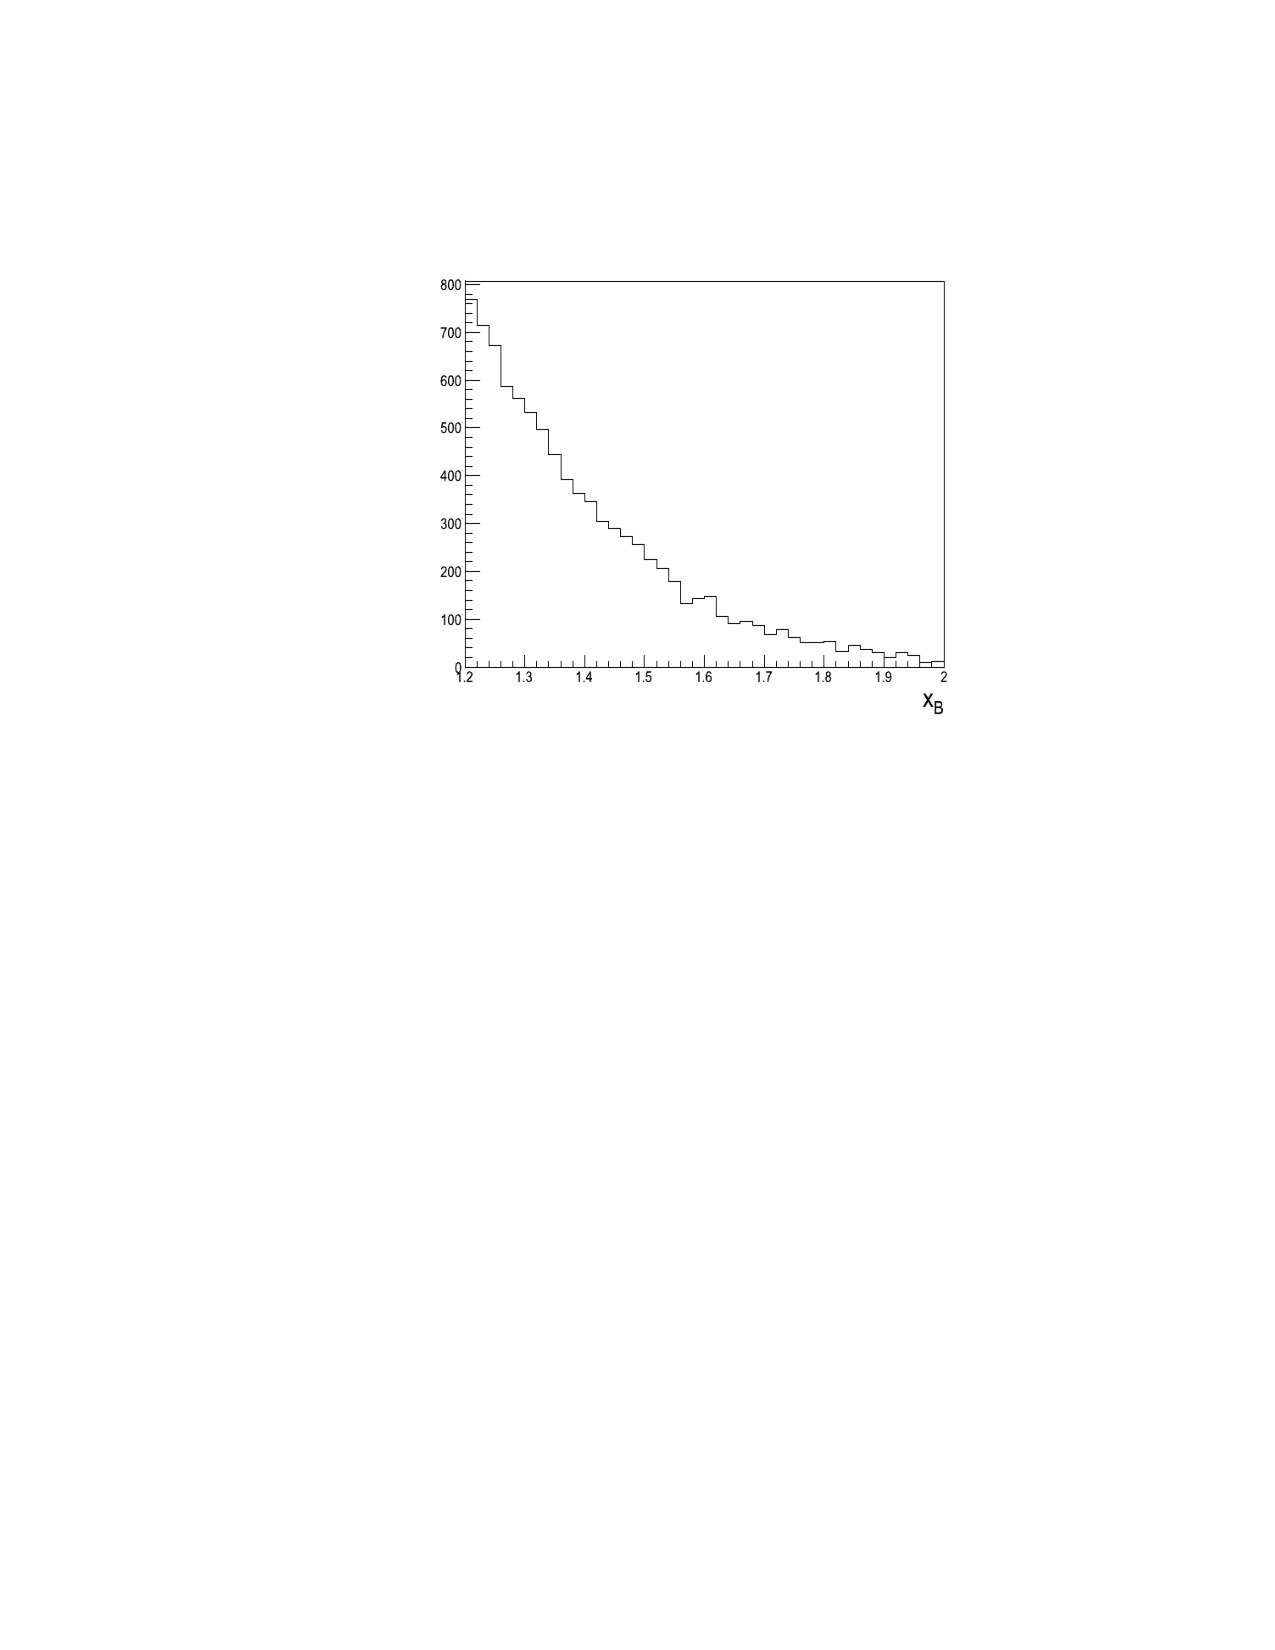
\includegraphics[width=0.43\textwidth]{or_note_figs/xB.pdf}
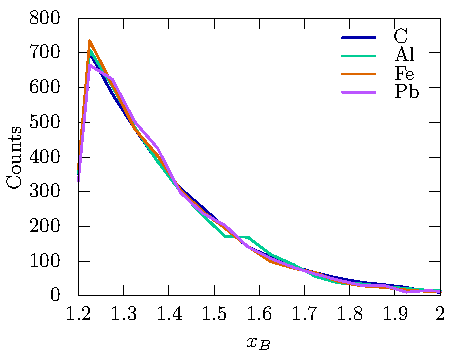
\includegraphics[width=0.49\textwidth]{leading_dist/leading_xB.pdf}\\
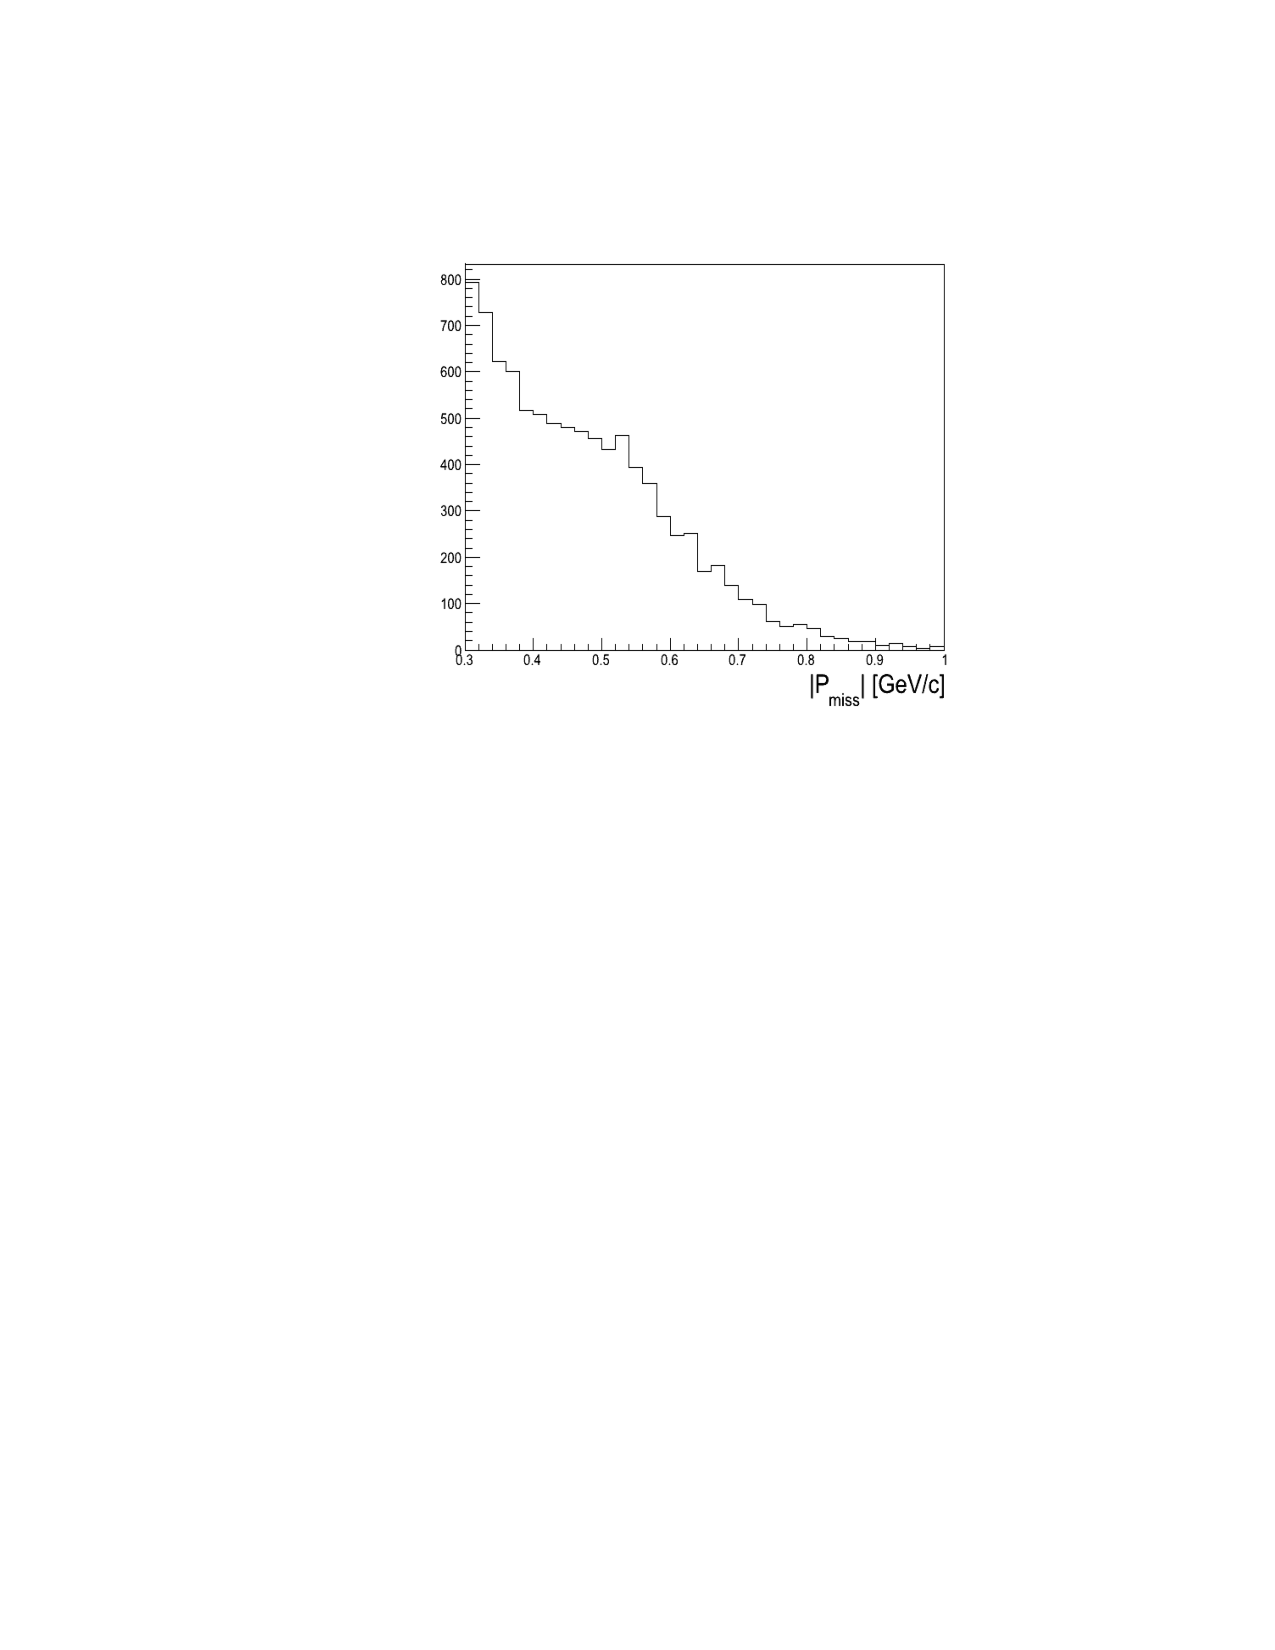
\includegraphics[width=0.43\textwidth]{or_note_figs/pm.pdf}
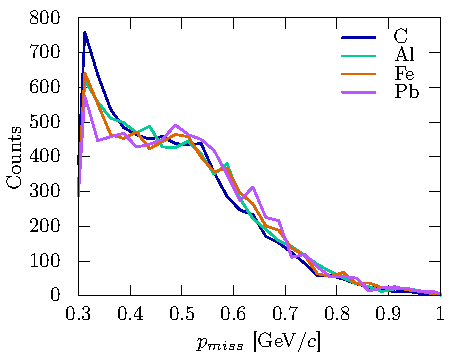
\includegraphics[width=0.49\textwidth]{leading_dist/leading_Pmiss.pdf}
\caption[Leading proton distributions]{
The leading protons have very similar kinematic distributions for all four nuclei.
Shown here are $Q^2$ (top), $x_B$ (middle), $p_\text{miss}$ (bottom). The left column
has figures from \cite{Or:note} for events from C, while the right columns has figures from this analysis,
from all four targets, including proton fiducial cuts. The data from the Al, Fe, and Pb
targets have been scaled to match the number of C events. 
\label{fig:leading}}
\end{figure}

Select kinematic distributions of leading protons are shown in figure \ref{fig:leading}.
As can be seen, the distributions are nearly identical for the four targets. 

%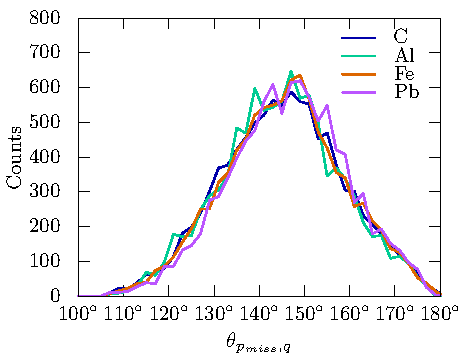
\includegraphics[width=0.49\textwidth]{leading_dist/leading_theta_Pmq.pdf}

Figure \ref{fig:ep_pm_e1} shows the correlation between the missing momentum and the initial
proton energy, defined by $E_p - \omega$. 

\begin{figure}[htpb]
\centering
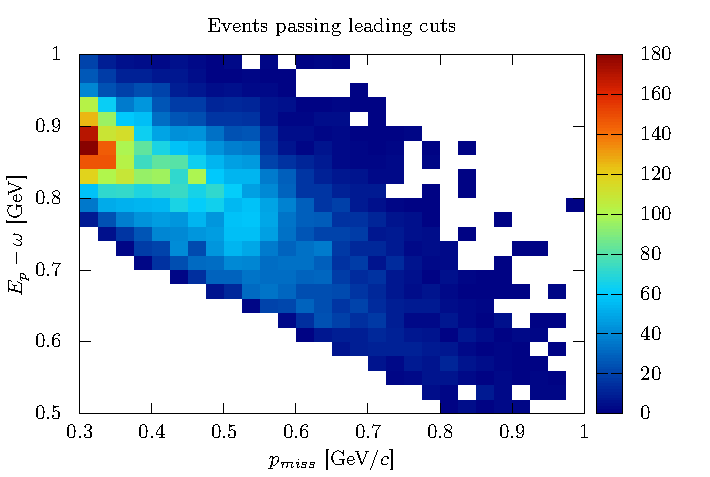
\includegraphics{pmiss_e1_ep.pdf}
\caption[Leading proton $p_\text{miss}$ vs. $E_1$]{
The leading protons show strong correlation between missing momentum
and $E_p - \omega$ (shown here for the carbon target), which should
be the case for the hard knockout of high-momentum protons.
\label{fig:ep_pm_e1}}
\end{figure}

\subsection{$A(e,e'pp)$ events}

The number of events passing both leading and recoil cuts is shown in table \ref{tab:recoil}

\begin{table}[h]
\centering
\begin{tabular}{c c c c c}
\hline
\hline
$p_\text{miss}$ [GeV$/c$] & C Events & Al Events & Fe Events & Pb Events\\
\hline
0.3--0.4  &  26 &  7 &  28 &  1 \\
0.4--0.5  &  96 & 35 &  61 & 15 \\
0.5--0.6  & 128 & 39 & 124 & 25 \\
0.6--0.7  & 102 & 39 & 111 & 31 \\
0.7--0.8  &  58 & 15 &  62 & 11 \\
0.8--0.9  &  21 &  9 &  22 &  4 \\
0.9--1.0  &   6 &  2 &  14 &  2 \\
\hline
Total & 437 & 146 & 422 & 89 \\
\hline
\end{tabular}
\caption{\label{tab:recoil} Events passing both leading and recoil proton cuts; the numbers
of events is smaller than in Table VII of \cite{Or:note} because of the additional proton
fiducial cuts.}
\end{table}

\begin{figure}[htpb]
\centering
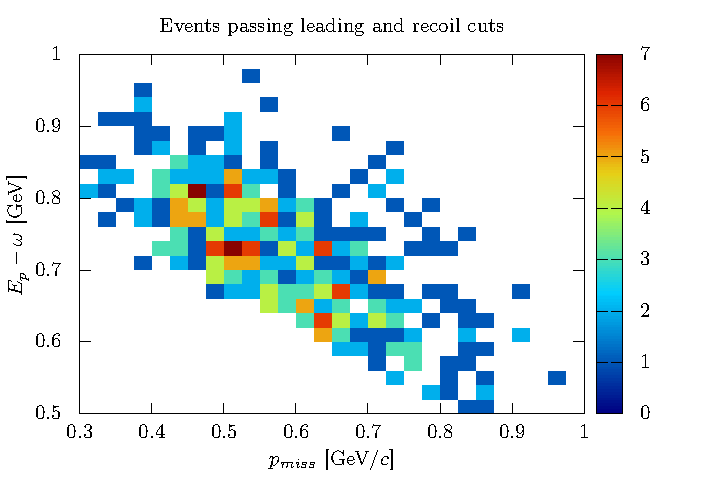
\includegraphics{pmiss_e1_epp.pdf}
\caption[Two proton $p_\text{miss}$ vs. $E_1$]{
The leading protons from $e'pp$ events also show strong correlation 
between missing momentum and $E_p - \omega$ (shown here for the carbon target).
\label{fig:epp_pm_e1}}
\end{figure}


\section{Comparing Simulation to Data}
\label{sec:comp}

We have developed a new Monte Carlo event generator based on Generalized Contact
Formalism (GCF), a formalism described in ref.~\cite{weiss:2016obx}. 
This generator allows the simulation of the reaction shown in figure \ref{fig:reaction}, 
in which an electron has a hard scattering from a nucleon in a short-range correlated (SRC)
pair within a nucleus, causing both the struck nucleon and the correlated partner nucleon
to be ejected from the nucleus. The generator produces a list of events, each containing 
momentum vectors for a scattered electron, a leading nucleon, and a recoil nucleon, as 
well as a cross section weight, include radiative corrections
(adapting the peaking approximation approach laid out in \cite{Ent:2001hm}).

To compare our event generator to data, we use the following steps:
\begin{itemize}
\item Generate Monte Carlo events,
\item Weight events by the simulated CLAS acceptance,
\item Smear generated electron and proton momenta,
\item Reject particles outside of the fiducial region,
\item Apply same event selection cuts used on the data.
\end{itemize}

We produced CLAS acceptance maps, using the same procedure
as in the approved analyses of refs.~\cite{Meytal:note} and \cite{Erez:note}. 
For this work, we produced maps with finer binning. The acceptance for 
1~GeV$/c$ protons is shown in \ref{fig:maps}.

\begin{figure}[htpb]
\centering
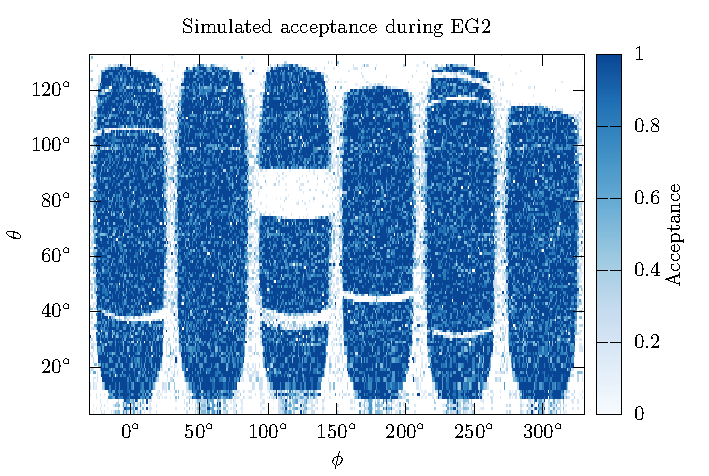
\includegraphics{maps.pdf}
\caption[Acceptance Map]{The acceptance map for 1~GeV$/c$ protons from the solid target position is shown,
with the six CLAS sectors clearly visible, as well as gaps caused by non-functioning
scintillator paddles.
\label{fig:maps}
}
\end{figure}

We accounted for resolution by smearing the magnitude of generated particle momentum vectors.
We chose the following resolutions (with the uncertainty varied as a systematic effect).
\begin{itemize}
\item Electrons: $0.3\% \pm 0.05\%$
\item Protons: $1.0\% \pm 0.20\%$
\end{itemize}

We accounted for the final state effects of transparency and single-charge exchange (SCX)
using:
\begin{equation}
\begin{split}
\sigma^{Exp}_{A(e,e'pp)} = &\sigma^{GCF}_{A(e,e'pp)} \cdot P_{A}^{pp}\cdot T_{A,pp} + \\
 & \sigma^{GCF}_{A(e,e'np)}\cdot p_{A}^{[n]p}\cdot T_{A}^{*} + \\
 & \sigma^{GCF}_{A(e,e'pn)}\cdot P_{A}^{p[n]}\cdot T_{A}^{*}, \\ \\
\sigma^{Exp}_{A(e,e'p)} = & (\sigma^{GCF}_{A(e,e'pp)} + \sigma^{GCF}_{A(e,e'pn)}) \cdot P_{A}^{p}\cdot T_{A,p} + \\
 & \sigma^{GCF}_{A(e,e'np)} \cdot P_{A}^{[n]p}\cdot T_{A}^{*} + \\
 &\sigma^{GCF}_{A(e,e'nn)}\cdot P_{A}^{[n]n}\cdot T_{A}^{*},
\end{split}
\label{eq:scx_gcf}
\end{equation}
where $\sigma^{GCF}_{X}$ is the GCF calculated cross-section for process X without FSI.

Uncertainty on the CLAS resolution factors, transparency factors, SCX probabilities, 
as well as many other parameters internal to the event generator,
contribute systematic uncertainty. Our approach was to simulate a large number of 
``universes'', in which the uncertain parameters are each randomly drawn from a prior probability
distribution. We then examine the spread of the generator results across this space
of universes to produce a systematic uncertainty band.

\begin{figure}[htpb]
\centering
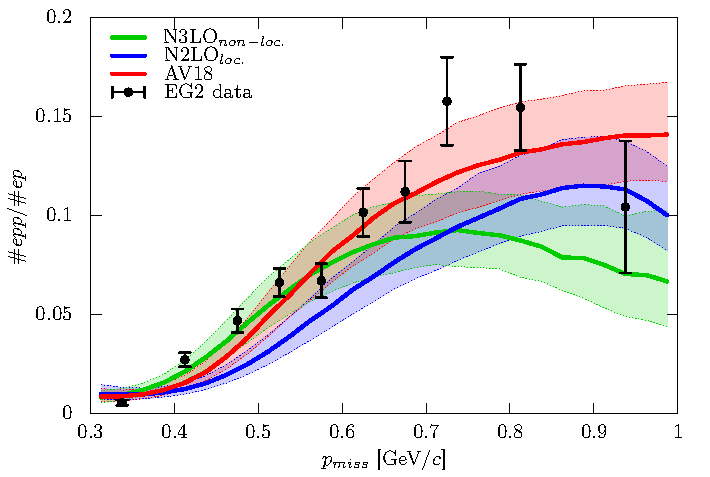
\includegraphics[width=12cm]{pp2p.pdf}
\caption[$e'pp/e'p$]{The ratio of $e'pp$ events to $e'p$ events from this analysis can 
provide a constraint on $NN$ potentials.
\label{fig:pp2p}
}
\end{figure}

Figure~\ref{fig:pp2p} shows the signature result of this analysis, the ratio of
$A(e,e'pp)$ events to $A(e,e'p)$ events as a function of missing momentum. The data
are shown as black points, compared with the predictions from the Monte Carlo event
generator using three different $NN$ interactions as input: AV18 (red), a local N2LO chiral (blue)
potential, and a non-local N3LO chiral potential (green). The 68\% confidence intervals
from the simulation due to systematic effects are shown in the light shaded bands. 
Shown here are the results from the carbon target, where the theoretical inputs are
best constrained. Both the theory and simulation show an increasing trend in the
fraction of $e'pp$ events, but different $NN$ potentials predict different shapes
for that trend, and the data favor a steeper transition, agreeing best with AV18. 

Further data-theory comparisons are appended to this note.

\bibliographystyle{ieeetr}
\bibliography{references}

\clearpage
\includepdf[pages=2-6]{jackson_report.pdf}


\end{document}
